\documentclass[conference]{IEEEtran}
\usepackage[utf8]{inputenc}
\usepackage[english]{babel}
\usepackage{graphicx}
\usepackage{float}
\usepackage{hyperref}
\usepackage{booktabs}
\usepackage{array}
\usepackage{amsmath}

\usepackage{tikz}
\usetikzlibrary{shapes.geometric, arrows.meta, positioning, fit, backgrounds}

\hypersetup{
    colorlinks=true,
    linkcolor=blue,
    urlcolor=blue,
    citecolor=black
}

\begin{document}

\title{System Design Document: \\ Software-Defined Campus Energy Management (Proof of Concept)}

\author{
\IEEEauthorblockN{Omar Yesid Fonseca López, Daniel Felipe Barrera Suárez, \\ Daniel Mateo Ballesteros Molina, Dania Lizeth Guzmán Triviño}
\IEEEauthorblockA{\textit{Systems Engineering Program} \\
\textit{Universidad Distrital Francisco José de Caldas}\\
Bogotá, Colombia \\
\{oyfonsecal, dfbarreras, dmballesterosm, dlguzmant\}@udistrital.edu.co}
}

\maketitle

\begin{abstract}
High energy consumption in university facilities, largely driven by unoccupied laboratories with active computing equipment, presents a critical sustainability challenge constrained by strict institutional IT security policies. To address this, we propose a decentralized, software-defined Proof of Concept (PoC) utilizing autonomous user-space telemetry agents, cloud-based data storage, and behavioral nudges. This approach bypasses the need for physical IoT infrastructure or administrator privileges, providing a highly feasible, secure, and scalable solution to optimize energy usage and reduce institutional waste.
\end{abstract}

\begin{IEEEkeywords}
Energy Management, Autonomous Telemetry, Proof of Concept, Python, User-Space, Smart Campus
\end{IEEEkeywords}

\section{Introduction}
The initial systems analysis (Workshop \#1) of the Engineering Faculty laboratories revealed a critical inefficiency: computing equipment and lighting are frequently left active during unoccupied hours due to human negligence \cite{b1}. Previous approaches to similar problems often rely on centralized physical IoT sensor networks or direct hardware interventions. Indeed, research indicates that occupant behavior significantly impacts building energy consumption, sometimes increasing it by up to 150\% \cite{b2}. However, implementing traditional hardware solutions in public university settings presents severe logistical and financial barriers. Furthermore, institutional IT policies strictly prevent the use of private perimeter networks, centralized orchestration servers, or the installation of software requiring administrator privileges on laboratory workstations.

To ensure practical feasibility within these boundaries, this document presents a Software-Defined Energy Management design that operates strictly as an academic Proof of Concept (PoC). By leveraging non-privileged OS-level scripts, the system autonomously evaluates inactivity on each machine, alerts administrators via public APIs (Telegram), and executes local suspensions. This methodology aims to achieve the university's sustainability goals without altering its existing physical or network infrastructure.

\section{Requirements Analysis}

\subsection{Synthesis of Workshop \#1 Findings}
The data collection phase highlighted that technological solutions must account for both human behavior and IT roadblocks. Table \ref{tab:findings} summarizes these insights.

\begin{table}[htbp]
\caption{Key Findings and Constraints from Phase 1}
\label{tab:findings}
\centering
\begin{tabular}{|p{3cm}|p{4.5cm}|}
\hline
\textbf{Analytical Finding} & \textbf{System Implication / Constraint} \\
\hline
High frequency of equipment waste & Automated idle detection is required on every PC. \\
\hline
Awareness-Action Gap & 80\% of users forget to power down; behavioral nudges are needed. \\
\hline
Strict IT Security & Mandatory execution without local administrator rights. \\
\hline
Limited Infrastructure & Absence of a central server for orchestration. \\
\hline
\end{tabular}
\end{table}

\subsection{Design Requirements}
Translating the analytical findings into measurable engineering specifications results in the requirements outlined in Table \ref{tab:requirements}.

\begin{table}[htbp]
\caption{System Design Requirements}
\label{tab:requirements}
\centering
\begin{tabular}{|c|p{2.5cm}|p{4cm}|}
\hline
\textbf{ID} & \textbf{Requirement} & \textbf{Metric / Criterion} \\
\hline
R-01 & Autonomous Execution & The agent must operate without relying on local network servers. \\
\hline
R-02 & Safe Detection & Accurately identify $>15$ minutes of no input via standard APIs. \\
\hline
R-03 & Local Suspension & Invoke OS Suspend (\textit{Sleep}) states instead of forced shutdowns. \\
\hline
R-04 & External Communication & Send logs via HTTPS or save to a local CSV file. \\
\hline
\end{tabular}
\end{table}

\section{System Architecture Design}

\subsection{Component and Module Description}
To comply with the strict constraints, the architecture is simplified into independent nodes that collect, process, and act upon their own data, as illustrated in Fig. \ref{fig:arch}. The Perception and Processing Layer consists of an Autonomous Agent, built as a Python executable residing in the user's startup folder, which monitors idle time and executes business logic internally. The Network Layer employs a unidirectional messaging API (Telegram) to notify the project team of system activations. For the Data Layer, a cloud-based MySQL database is utilized, with a fallback mechanism to a local CSV file in the event of firewall blocking. Finally, the Application Layer uses Power BI dashboards connected to the data source to generate project viability reports.

\begin{figure}[htbp]
\centering
\resizebox{\columnwidth}{!}{
\begin{tikzpicture}[
    node distance=2cm and 3cm,
    box/.style={draw, rectangle, minimum width=3cm, minimum height=1.2cm, align=center, fill=blue!10, rounded corners},
    db/.style={draw, cylinder, shape border rotate=90, aspect=0.25, minimum height=1.5cm, minimum width=2.2cm, align=center, fill=orange!10},
    arrow/.style={->, >=stealth, thick}
]


\node[box] (agent) {Autonomous Agent \\ (Python .exe)};
\node[box, below=1.5cm of agent] (os) {Local OS APIs \\ (ctypes, psutil)};


\begin{scope}[on background layer]
    \node[fill=gray!10, draw=gray, dashed, fit=(agent) (os), inner xsep=0.8cm, inner top sep=1.2cm, inner bottom sep=0.6cm] (pc) {};
    \node[anchor=north, yshift=-0.2cm] at (pc.north) {\textbf{Local Workstation (User-Space)}};
\end{scope}

\node[box, right=3cm of agent, yshift=1.5cm] (telegram) {Telegram API \\ (Alerts)};
\node[db, right=3cm of agent, yshift=-1.5cm] (mysql) {MySQL DBaaS \\ (Cloud)};
\node[box, right=2cm of mysql] (powerbi) {Power BI \\ (Dashboard)};
\draw[arrow, <->] (agent) -- node[right] {Telemetry} (os);
\draw[arrow] (agent.east) -- node[above, sloped] {HTTPS (Outbound)} (telegram.west);
\draw[arrow] (agent.east) -- node[above, sloped] {HTTPS / Local CSV} (mysql.west);
\draw[arrow] (mysql.east) -- node[above] {Query} (powerbi.west);

\end{tikzpicture}%
}
\caption{Decentralized Software-Defined System Architecture}
\label{fig:arch}
\end{figure}

\subsection{Data Flow and Operational Logic}
The operational logic follows a sequential evaluation loop depicted in Fig. \ref{fig:flow}. Initially, the Autonomous Agent reads the OS idle time every minute. Upon detecting fifteen minutes of inactivity, the system deploys a behavioral nudge, displaying a deterrent full-screen overlay that asks the user to interact with the machine if it is still in use. If there is no interaction within sixty seconds, the PC safely enters sleep mode. Consequently, the "Savings Activated" state is transmitted to the cloud via HTTPS or written to the local CSV file to ensure data persistence.

\begin{figure}[htbp]
\centering
\resizebox{0.85\columnwidth}{!}{%
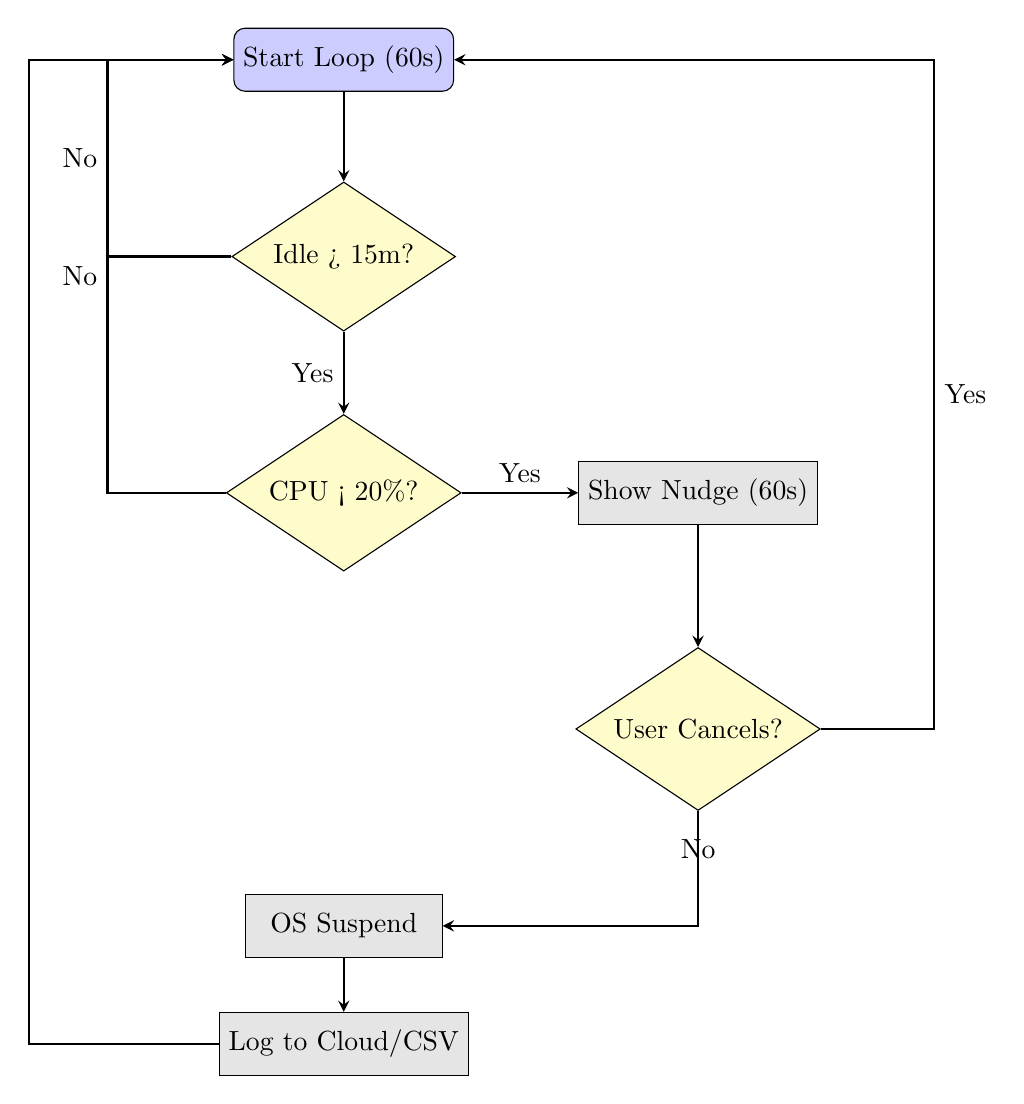
\begin{tikzpicture}[
    node distance=1.5cm,
    startstop/.style={rectangle, rounded corners, minimum width=2cm, minimum height=0.8cm, text centered, draw=black, fill=blue!20},
    process/.style={rectangle, minimum width=2.5cm, minimum height=0.8cm, text centered, draw=black, fill=gray!20},
    decision/.style={diamond, minimum width=2.5cm, minimum height=0.8cm, text centered, draw=black, fill=yellow!20, aspect=1.5},
    arrow/.style={thick,->,>=stealth}
]

\node (start) [startstop] {Start Loop (60s)};
\node (idle) [decision, below of=start, yshift=-1cm] {Idle > 15m?};
\node (cpu) [decision, below of=idle, yshift=-1.5cm] {CPU < 20\%?};
\node (nudge) [process, right of=cpu, xshift=3cm] {Show Nudge (60s)};
\node (cancel) [decision, below of=nudge, yshift=-1.5cm] {User Cancels?};
\node (suspend) [process, below of=cpu, yshift=-4cm] {OS Suspend};
\node (log) [process, below of=suspend] {Log to Cloud/CSV};


\draw [arrow] (start) -- (idle);
\draw [arrow] (idle) -- node[anchor=east] {Yes} (cpu);
\draw [arrow] (idle) -- ++(-3,0) |- node[anchor=east, near start] {No} (start);
\draw [arrow] (cpu) -- node[anchor=south] {Yes} (nudge);
\draw [arrow] (cpu) -- ++(-3,0) |- node[anchor=east, near start] {No} (start);
\draw [arrow] (nudge) -- (cancel);
\draw [arrow] (cancel) -- ++(3,0) |- node[anchor=west, near start] {Yes} (start);
\draw [arrow] (cancel) |- node[anchor=south, near start] {No} (suspend);
\draw [arrow] (suspend) -- (log);
\draw [arrow] (log) -- ++(-4,0) |- (start);

\end{tikzpicture}%
}
\caption{Autonomous Agent Operational Workflow and Decision Logic}
\label{fig:flow}
\end{figure}

\section{Technical Implementation Strategy}

\subsection{Justification of Selected Technologies}
The selected technologies prioritize a clean deployment that bypasses traditional IT hurdles. Compiling the Python script into a standalone executable via PyInstaller entirely eliminates the need to install the Python interpreter on university machines. For data management, utilizing a cloud-based MySQL database alongside a local CSV fallback allows for robust data persistence without provisioning internal server infrastructure. Finally, Microsoft Power BI facilitates processing these data sources to deliver professional, executive-level visualizations for the final project delivery.

\subsection{Implementation Phases (Academic PoC)}
The scope is strictly defined as a controlled academic pilot test. The first phase consists of prototyping the Python agent and conducting local testing on the research team's personal laptops. Subsequently, the pilot phase involves the manual installation of the executable on a small sample of lab computers, strictly with the instructor's permission. The data collection phase will run for two weeks, utilizing either cloud review or manual extraction of CSV files. The project will conclude with the consolidation of this data in Power BI and the drafting of the estimated energy savings report.

\section{Complexity and Risk Mitigation}

\subsection{Data Loss Prevention (Computational Load)}
In an engineering environment, peripheral inactivity does not necessarily equal processing inactivity, as tasks like 3D rendering or heavy compiling often run unattended. Suspending the equipment under these circumstances would catastrophically ruin the student's work. To mitigate this risk, the Autonomous Agent incorporates a complexity validation process. Before launching the behavioral nudge, the script verifies the processor's usage. If the CPU load exceeds $20\%$, the system safely assumes a critical background process exists, resets the inactivity timer, and aborts the suspension sequence entirely.

\subsection{Resilience Against Firewall Restrictions}
University perimeter policies often block outbound HTTPS requests to external APIs like Telegram or non-institutional databases. To address this network complexity, the agent is designed with structured exception handling. If network requests fail due to a firewall, the agent prioritizes its primary objective of suspending the equipment and stores the event locally in an encrypted log file. This ensures that the experimental data is preserved for later physical extraction via USB.

\section{Performance and Optimization Design}

\subsection{Success Metrics}
Given the nature of this Proof of Concept, system performance will be evaluated quantitatively using the metrics extracted from the generated logs, as detailed in Table \ref{tab:metrics}.

\begin{table}[htbp]
\caption{System Performance Metrics}
\label{tab:metrics}
\centering
\begin{tabular}{|p{2.5cm}|p{2cm}|p{3cm}|}
\hline
\textbf{Metric} & \textbf{PoC Goal} & \textbf{Measurement Method} \\
\hline
Agent Reliability & $>95\%$ Uptime & Difference between expected and recorded logs. \\
\hline
Energy Savings & $>20\%$ reduction & Sum of sleep hours $\times$ Average PC consumption. \\
\hline
Nudge Effectiveness & $<10\%$ forced & Count of cancellations vs. executed suspensions. \\
\hline
Precision & $0$ complaints & Reports of suspensions during active work. \\
\hline
\end{tabular}
\end{table}

\section{Conclusion and Next Steps}
Redesigning the system toward a purely Software-Defined Energy Management model at the user-space level comprehensively mitigates the barriers imposed by physical infrastructure constraints and institutional security policies. Utilizing an autonomous agent ensures the Proof of Concept can be executed safely, isolated, and without demanding IT department resources, thereby maintaining the analytical rigor required for the course project. The immediate next steps involve finalizing the Python code utilizing libraries such as \textit{ctypes} and \textit{psutil}, conducting thorough black-box testing, and securing formal authorization from a laboratory instructor for deployment.

\section*{Acknowledgments}
The authors would like to thank Eng. Carlos Andrés Sierra and the Universidad Distrital Francisco José de Caldas for their guidance and support throughout the systems analysis and design process.

\begin{thebibliography}{00}
\bibitem{b1} C. A. Sierra, ``Workshop No. 1: Systems Analysis,'' \textit{Systems Analysis \& Design Course}, Universidad Distrital Francisco José de Caldas, 2026.
\bibitem{b2} T. Hong, et al., ``Advances in research and applications of energy-related occupant behavior in buildings,'' \textit{Energy and Buildings}, vol. 116, pp. 694-702, 2016.
\end{thebibliography}

\end{document}